\chapter{Spatial Domain: \refmod}
\label{ch:ref-mod}

It was Xenakis' goal for the curved surfaces of the Philips Pavilion
to reduce the sonic contribution of sound reflections as much as
possible.\cite{philips1958} He knew that reflections and the resulting
comb filtering could impair intelligibility and localization of music
and sounds.  The pavilion was to have hundreds of loudspeakers, and an
elaborate custom sequencer electronically selected which speakers
Edgard Var\`{e}se's music played from. However, large concave surfaces
have a of focussing effect on acoustic
reflections,\cite{Vercammen2008} which can result in severe filtering
and phase cancellations. There is evidence that carefully constructed
curved surfaces such as stage shells can be effective for performers
of acoustic music.\cite{DAntonio1991} However, in the context of
loudspeaker playback, the advantages of curved surfaces over flat
(non-parallel) surfaces are ambiguous at best.\cite{Cox2006} When we
hear an acoustic sound reflection off a concave surface, the sound can
arrive at our ears in two possible states:
\begin{enumerate}
\item The path of the sound from the source to the reflecting surface
  to our ears is equidistant for each point on the reflecting
  surface. Ignoring any direct sound, the reflection arrives in-phase,
  and the surface acts as acoustic amplifier of the reflection.
\item The path of the sound from the source to the reflecting surface
  to our ears is slightly different for each point on the surface. All
  the reflections arrive out of phase with each other.
\end{enumerate}
Parabolic microphones\sidenote[][-32mm]{Parabolic microphones use a
  specially designed parabolic reflector that focuses sound arriving
  from one direction on the microphone capsule. Handheld models are
  commonly used in birdsong recording, and on the sidelines of
  football games. They typically have a diameter of two feet or less,
  and can capture sound up to 500 feet away. Due to the size of the
  reflector, commercial parabolic microphones cannot capture sounds
  below approximately 1kHz.}\cite{Davis1989}, and acoustic whispering
chambers\sidenote{A room built such that the walls are angled to
  direct sound from one corner to another. If two people stand in the
  correct spaces in a whispering chamber, they can clearly hear each
  other whispering even though they may be at opposite ends of the
  room.} fall into the first category. Both use surfaces that are
angled to reflect all sound emanating from one direction to converge
at a certain point. If a concave surface reflecting surfaces is not
carefully designed to focus sounds \textit{in phase} it is much more
likely that the sounds will arrive out of phase. The curves of the
Philips Pavilion probably created an \emph{unusual} acoustic space,
rather than a good space for critical listening. However, this may
have been advantageous to the project: Part of the spectacle was
seeing, hearing, and experiencing something completely unprecedented
and unlike anything else.

\section{Composing with Space}
\label{sec:composing-with-space}
If Xenakis had been able to model the reflections and compose them
directly into the piece, what would the tools be like? How can we make
the difference between in phase reflections and out of phase
reflections intuitive?  It we had tools available to compose with
acoustic reflections, how could we use controlled filtering
creatively, and what kind of music, and architectural spaces would we
make? The Xenakis inspired \refmod is tool for experimenting with
architectural acoustic lenses. In several ways, it is an abstraction
from real-world acoustics
\begin{enumerate}
\item It is simplified to two dimensions.
\item It is frequency independent. Real sufaces reflect only
  wavelengths much smaller than the size of the
  reflector.\cite{Zhixin2005}
\end{enumerate}


\begin{figure*}[]
  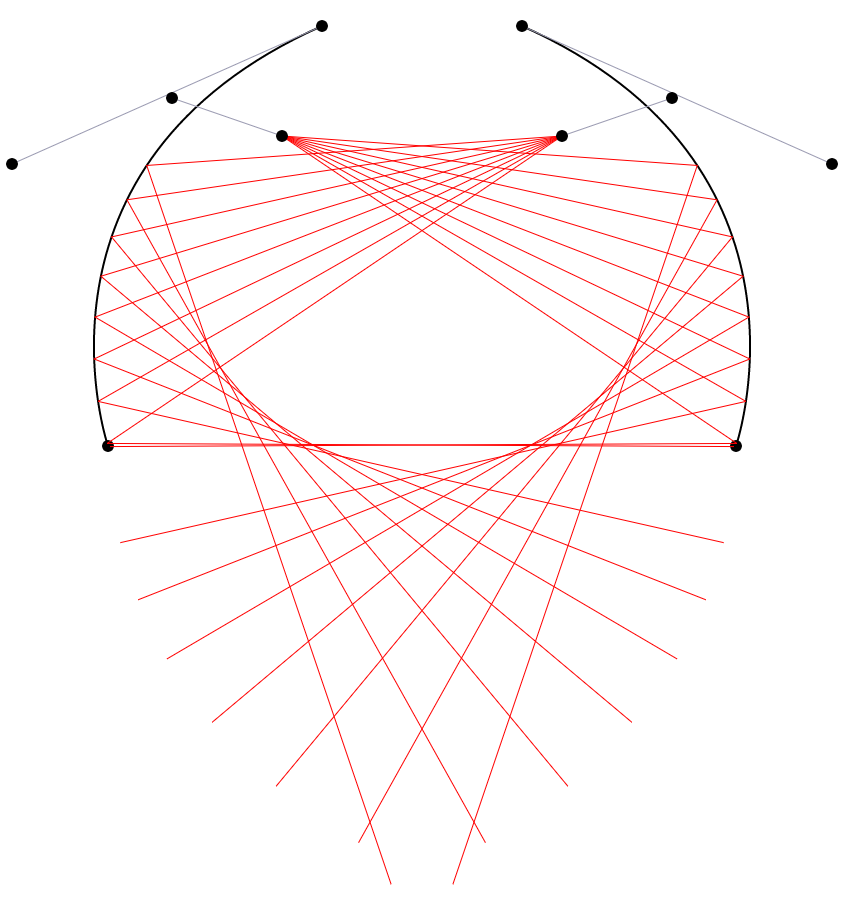
\includegraphics[width=\linewidth]{refmod/refmod.png}
  \caption[Tempo Transition]{\refmod user interface.}
  \label{fig:basic-tempo-change}
\end{figure*}


%%% Local Variables:
%%% mode: latex
%%% TeX-master: "CharlesHolbrow_MAS_Thesis"
%%% End:
